\chapter{Computer Arithmetic}


\section{Multiplication}

\subsection{Version 1}

\textbf{\textit{\#Question}:} \ {0010 * 0011}

\begin{multicols}{2}
   \begin{tabular}{|c|l|c|c|c|}\hline
      \thl{Itr} & \thl{Step} & \thl{Multiplier} & \thl{Multiplicand} & \thl{Product} \\\hline
      0 & Init & 0011 & 0000 0010 & 0000 0000 \\\hline
      % 
      1 & 1a & 001\red{1} & 0000 0010 & \red{0000 0010} \\
      & 2  & 0011 & \blue{0000 0100} & 0000 0010 \\
      & 3  & \blue{0001} & 0000 0100 & 0000 0010 \\\hline
      % 
      2 & 1a & 000\red{1} & 0000 0100 & \red{0000 0110} \\
      & 2  & 0001 & \blue{0000 1000} & 0000 0110 \\
      & 3  & \blue{0000} & 0000 1000 & 0000 0110 \\\hline
      % 
      3 & 1a & 000\red{0} & 0000 1000 & {0000 0110} \\
      & 2  & 0000 & \blue{0001 0000} & 0000 0110 \\
      & 3  & \blue{0000} & 0001 0000 & 0000 0110 \\\hline
      % 
      4 & 1a & 000\red{0} & 0001 0000 & {0000 0110} \\
      & 2  & 0000 & \blue{0010 0000} & 0000 0110 \\
      & 3  & \blue{0000} & 0010 0000 & 0000 0110 \\\hline
   \end{tabular}

   \vspace{1em}
   \begin{figure}[H]
      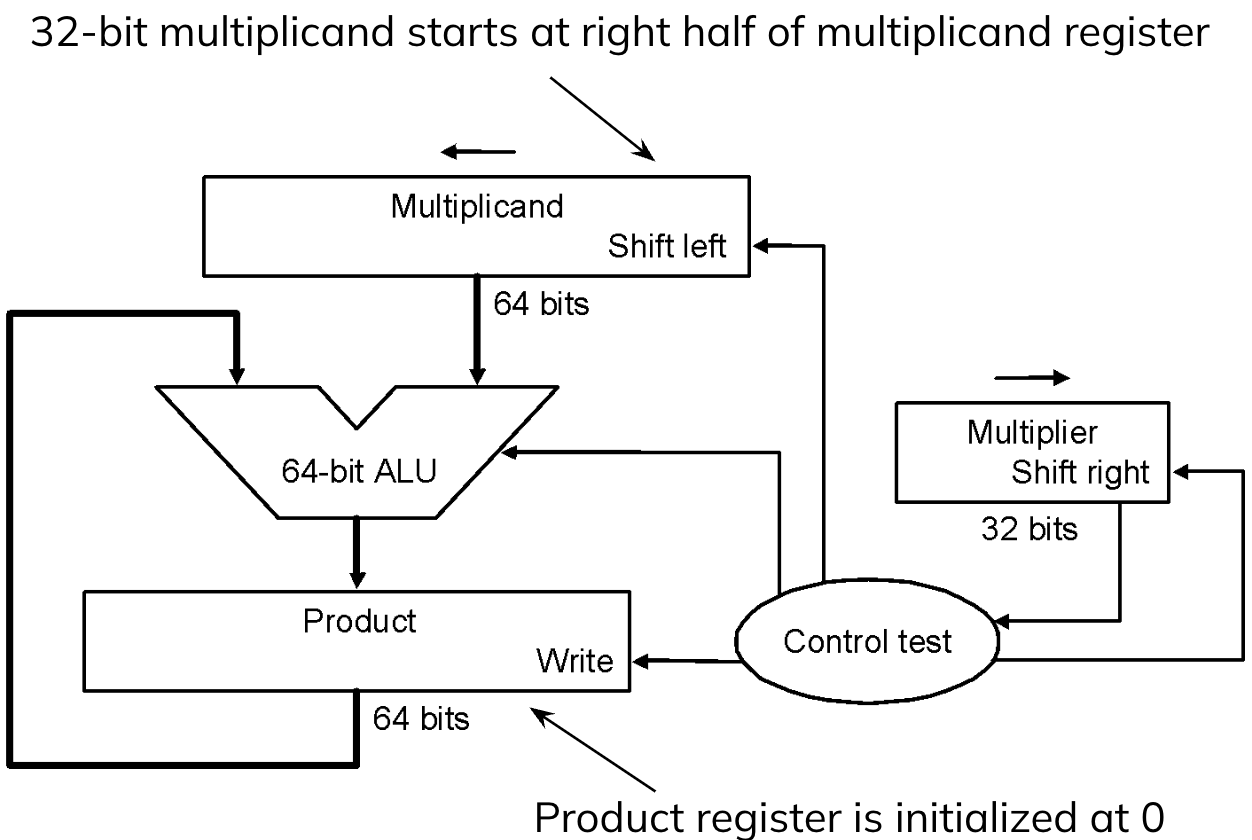
\includegraphics[width=0.45\textwidth]{figures/Multiplication V1.png}
   \end{figure}

   \columnbreak
   \begin{figure}[H]
      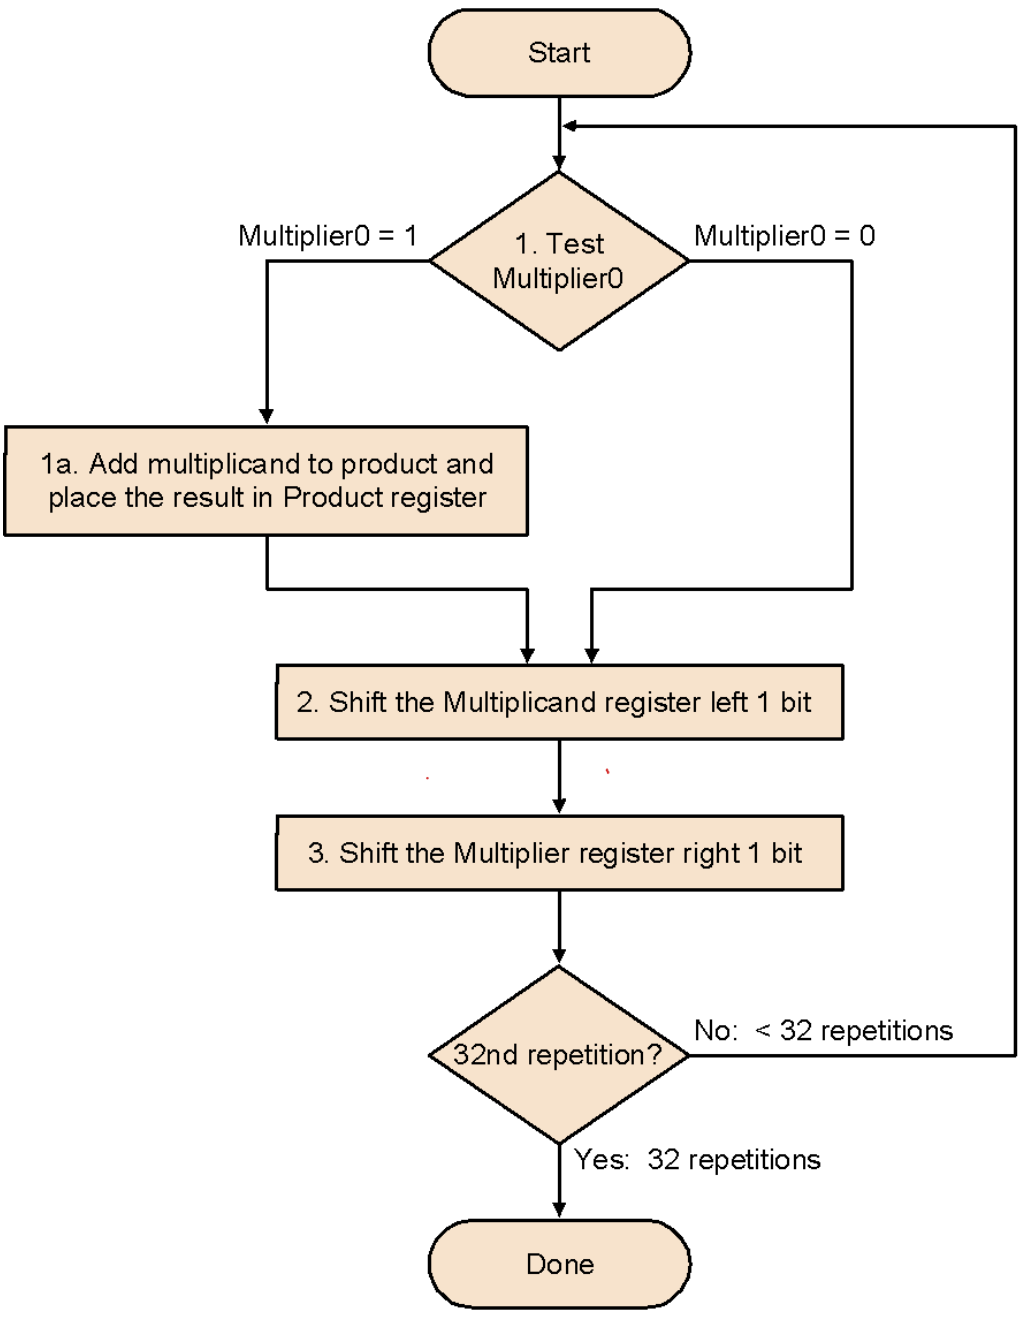
\includegraphics[width=0.45\textwidth]{figures/Multiplication V1 Algorithm.png}
   \end{figure}
\end{multicols}

\pagebreak
\subsection{Version 2}
\textbf{\textit{\#Question}:} \ {0010 * 0011}


\begin{multicols}{2}
   \begin{tabular}{|c|l|c|c|c|}\hline
      \thl{Itr} & \thl{Step} & \thl{Multiplier} & \thl{Multiplicand} & \thl{Product} \\\hline
      0 & Init & 0011 & 0010 & 0000 0000 \\\hline
      % 
      1 & 1a & 001\red{1} & 0010 & \red{0010} 0000\\
      & 2  & 0011 & 0010 & \blue{0001 0000} \\
      & 3  & \blue{0001} & 0010 & 0001 0000 \\\hline
      % 
      2 & 1a & 001\red{1} & 0010 & \red{0011} 0000\\
      & 2  & 0011 & 0010 & \blue{0001 1000} \\
      & 3  & \blue{0000} & 0010 & 0001 1000 \\\hline
      % 
      3 & 1a & 001\red{0} & 0010 & {0001 1000}\\
      & 2  & 0011 & 0010 & \blue{0000 1100} \\
      & 3  & \blue{0000} & 0010 & 0000 1100 \\\hline
      % 
      4 & 1a & 001\red{0} & 0010 & {0000 1100}\\
      & 2  & 0011 & 0010 & \blue{0000 0110} \\
      & 3  & \blue{0000} & 0010 & 0000 0110 \\\hline
   \end{tabular}

   \vspace{1em}
   \begin{figure}[H]
      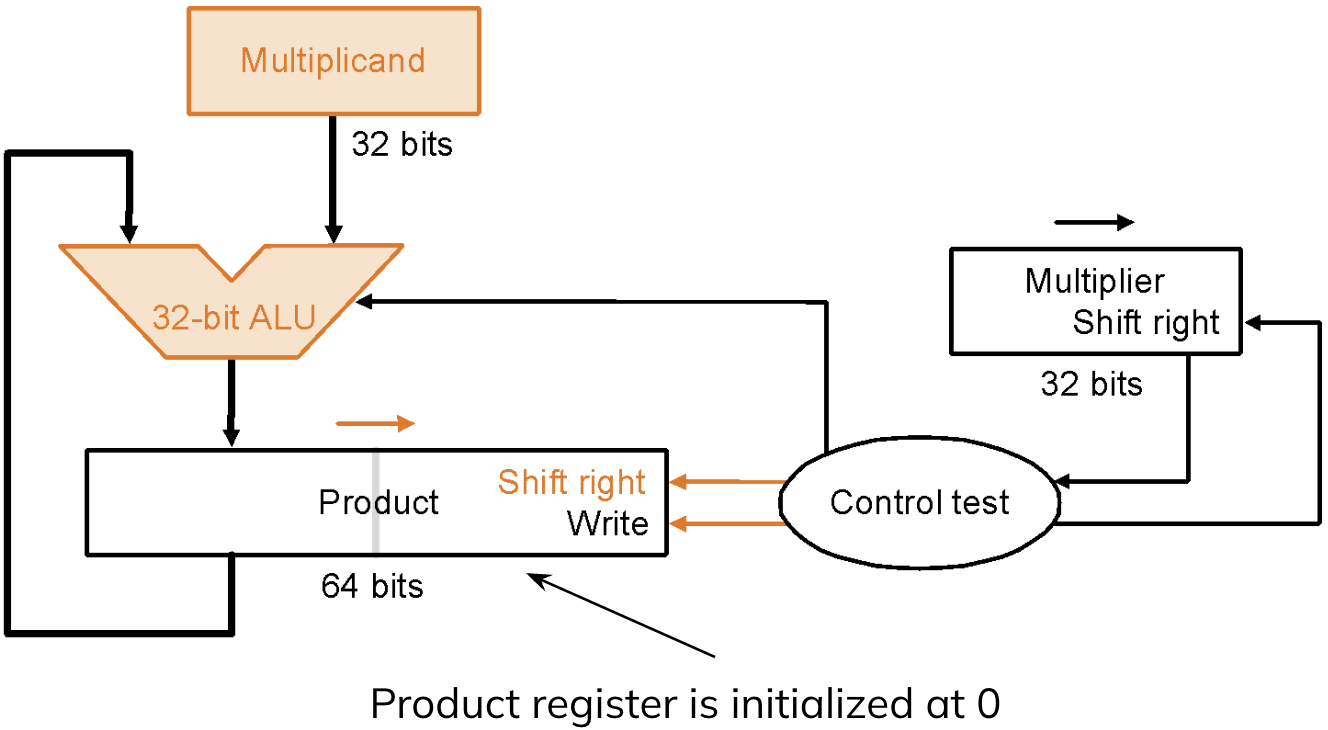
\includegraphics[width=0.45\textwidth]{figures/Multiplication V2.png}
   \end{figure}

   \columnbreak
   \begin{figure}[H]
      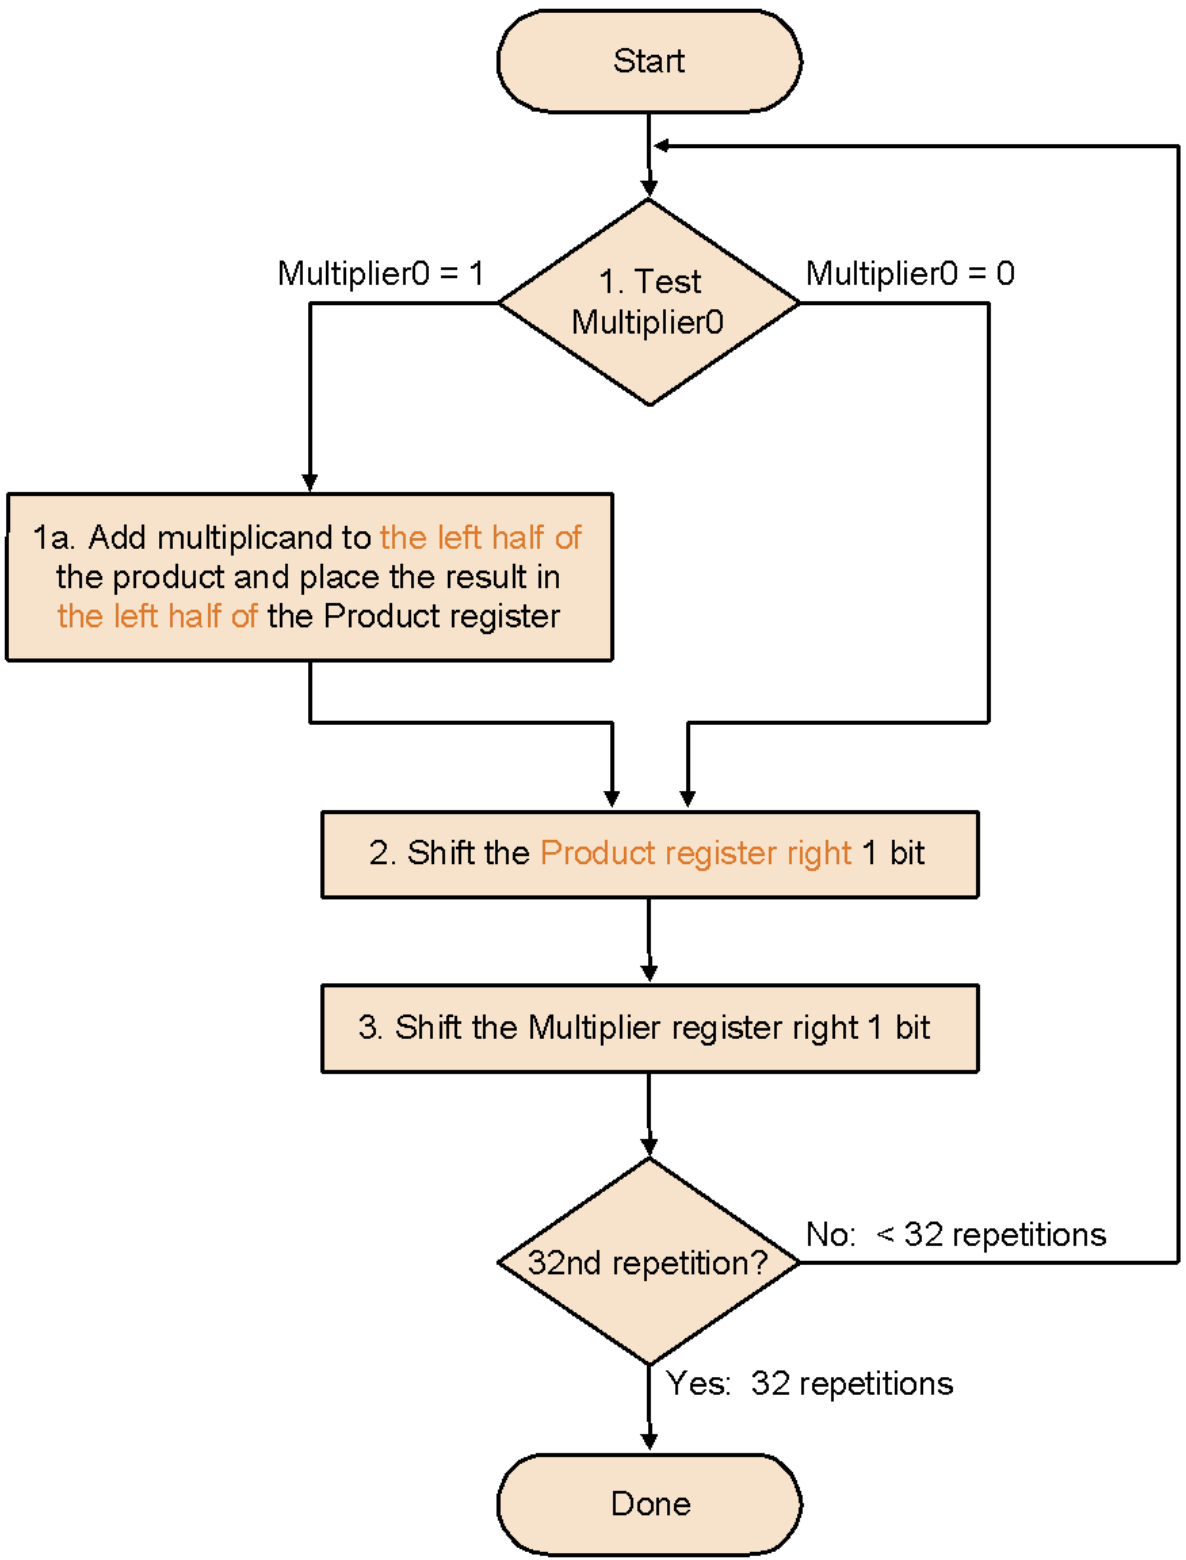
\includegraphics[width=0.45\textwidth]{figures/Multiplication V2 Algorithm.png}
   \end{figure}
\end{multicols}



\pagebreak
\subsection{Version 3}
\textbf{\textit{\#Question}:} \ {0100 * 0101}

\begin{multicols}{2}
   \begin{tabular}{|c|l|c|c|}\hline
      \thl{Itr} & \thl{Step} & \thl{Multiplicand} & \thl{Product} \\\hline
      0 & Init & 0100 & 0000 0101 \\\hline
      %
      1 & 1a & 0100 & \red{0100} 010\red{1}\\
      & 2  & 0100 & \blue{0010 0010} \\\hline
      %
      2 & 1a & 0100 & {0010} 001\red{0}\\
      & 2  & 0100 & \blue{0001 0001} \\\hline
      %
      3 & 1a & 0100 & \red{0101} 000\red{1}\\
      & 2  & 0100 & \blue{0010 1000} \\\hline
      %
      4 & 1a & 0100 & {0010} 100\red{0}\\
      & 2  & 0100 & \blue{0001 0100} \\\hline
   \end{tabular}

   \vspace{1em}
   \begin{figure}[H]
      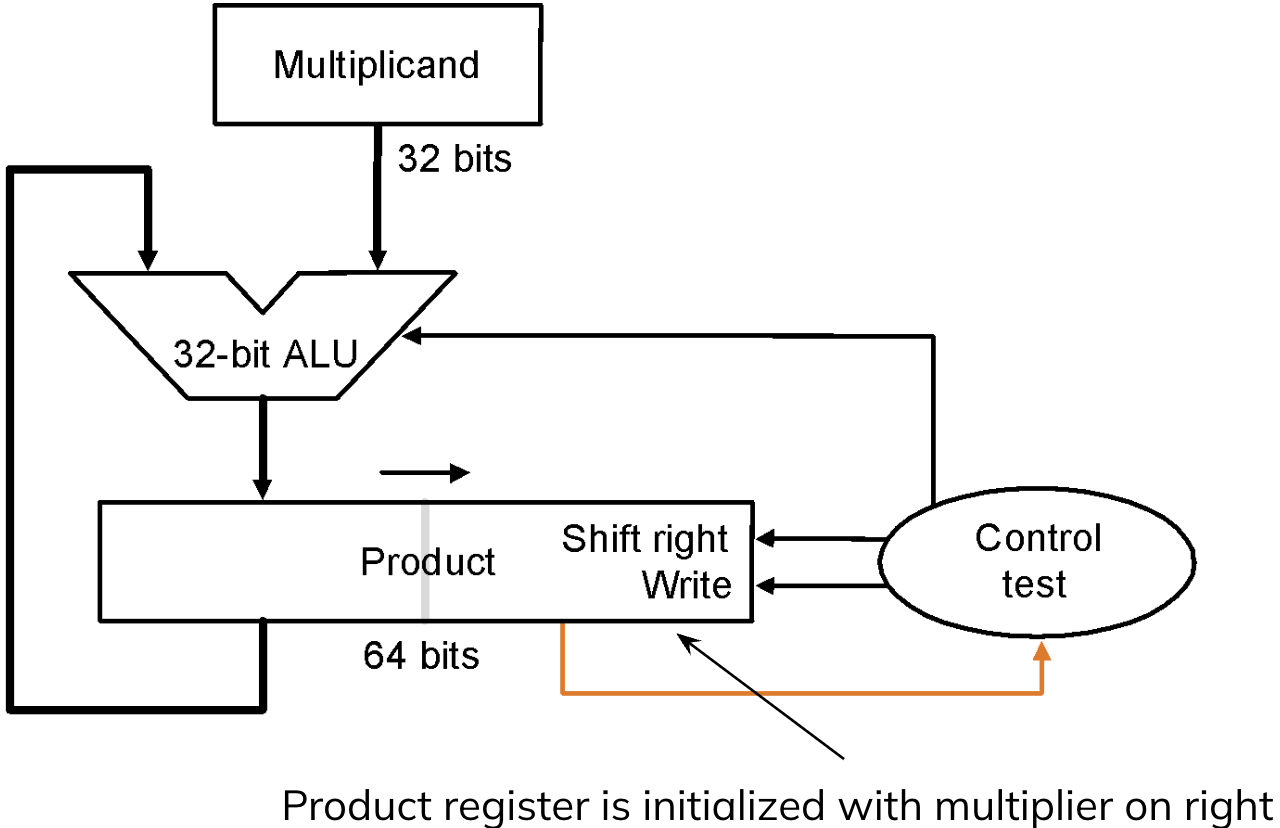
\includegraphics[width=0.45\textwidth]{figures/Multiplication V3.png}
   \end{figure}

   \columnbreak
   \begin{figure}[H]
      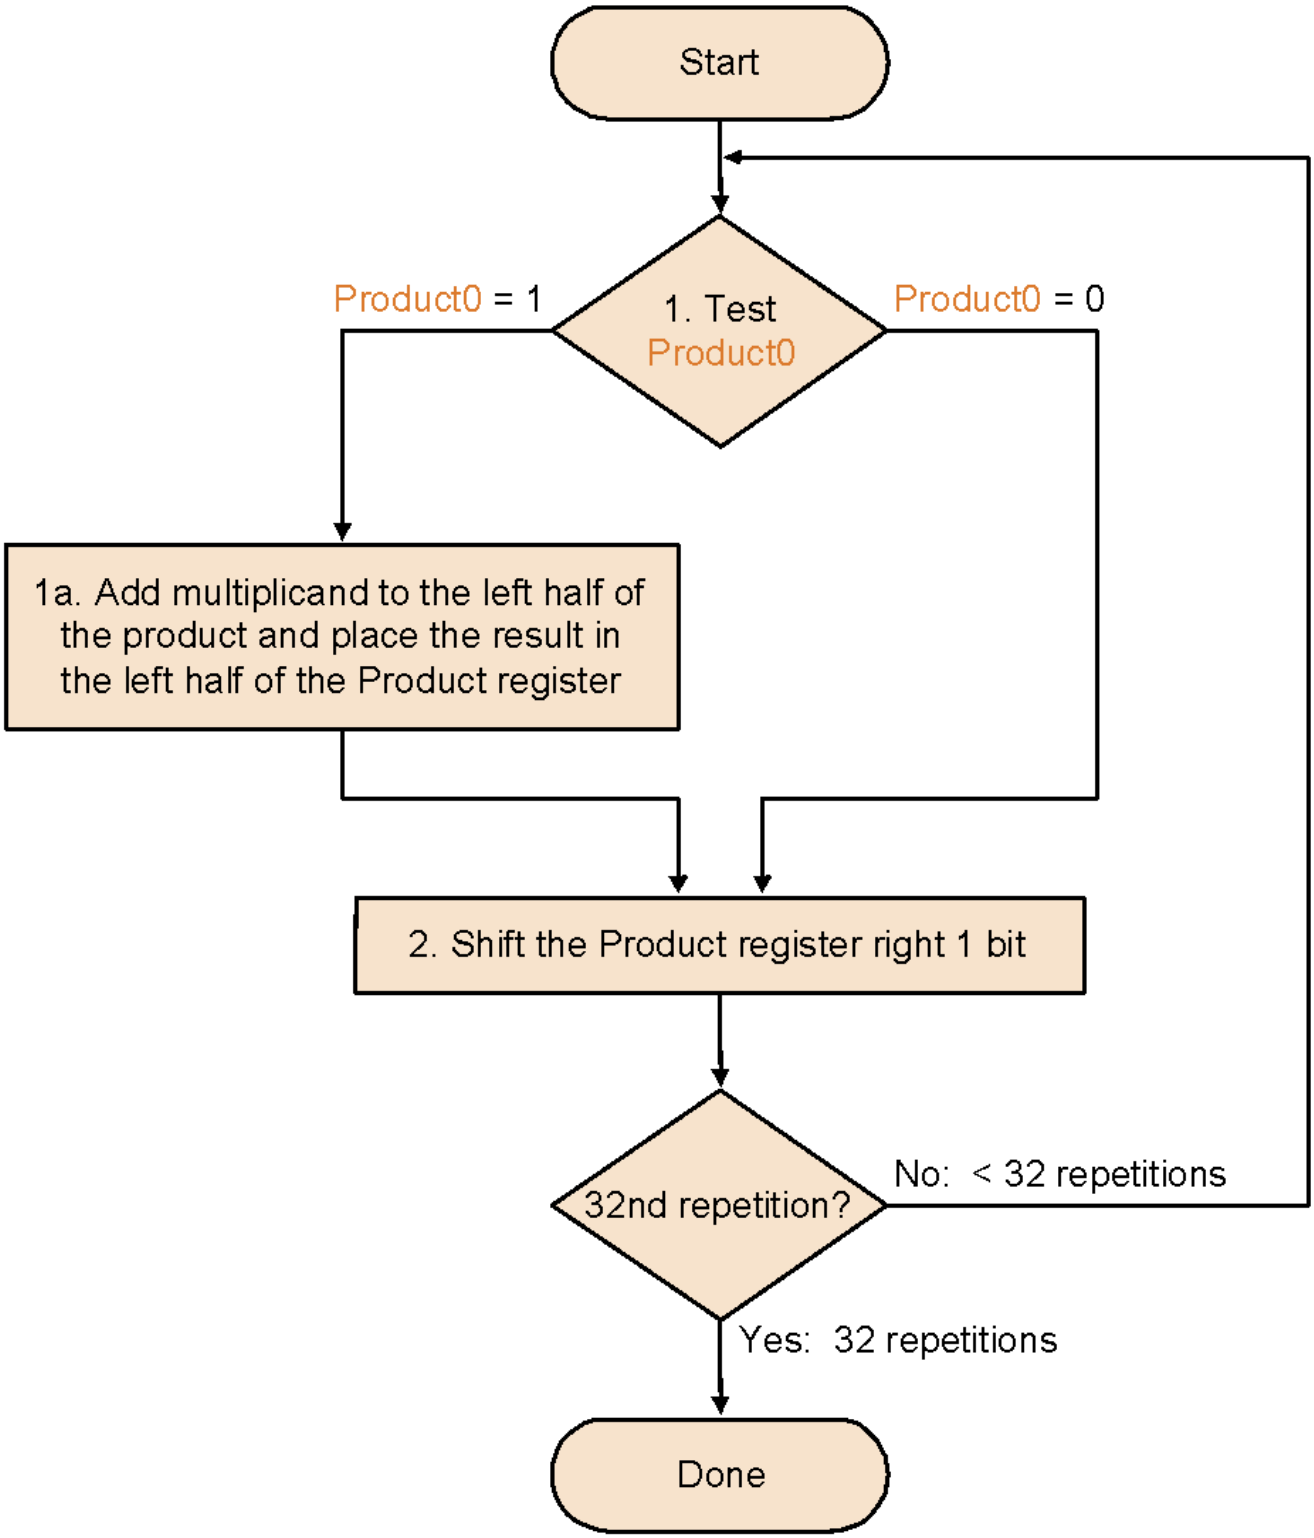
\includegraphics[width=0.45\textwidth]{figures/Multiplication V3 Algorithm.png}
   \end{figure}
\end{multicols}


\pagebreak
\subsection{Booth's Algorithm}
                     
\textbf{\textit{\#Question}:} \ {5 $\times$ -6}

\begin{minipage}[t]{0.65\textwidth}
   \vspace{0pt}
   \vtop{
   \begin{tabular}{|l|c|c|c|l|}\hline
      \thl{Operation} & \thl{Accumulator $(A)$} & \thl{Multiplier $(Q)$} & $Q_{-1}$ & \thl{Multiplicand $(M)$} \\\hline

      % Initial
      Init & 0 0 0 0 & 0 1 0 \red{1} & \red{0} &
      $\begin{array}{r}
         m = \text{1010} \\[-0.5em]
         -m = \text{0110}
      \end{array}$ \\\hline



      % Iteration-1
      \begin{tabular}{@{}l}
         $Q_0Q_{-1} = \text{10}$\\[-0.5em] Sub $m$\\[-0.5em] \textit{SAR}
      \end{tabular}
      &
      \begin{tabular}{c}
         0 1 1 0 \\\hline
         0 1 1 0 \\
         \blue{0} 0 1 1
      \end{tabular}
      &
      \begin{tabular}{c}
         \\0 1 0 1
         \\0 0 1 \red{0} 
      \end{tabular}
      & \begin{tabular}{c}
         \\\\\red{1}
      \end{tabular}&\\\hline



      % Iteration-2
      \begin{tabular}{@{}l}
         $Q_0Q_{-1} = \text{01}$\\[-0.5em] Add $m$\\[-0.5em] \textit{SAR}
      \end{tabular}
      &
      \begin{tabular}{c}
         1 0 1 0 \\\hline
         1 1 0 1 \\
         \blue{1} 1 1 0
      \end{tabular}
      &
      \begin{tabular}{c}
         \\0 0 1 0
         \\1 0 0 \red{1}
      \end{tabular}
      & \begin{tabular}{c}
         \\\\\red{0}
      \end{tabular}&\\\hline



      % Iteration-3
      \begin{tabular}{@{}l}
         $Q_0Q_{-1} = \text{10}$\\[-0.5em] Sub $m$\\[-0.5em] \textit{SAR}
      \end{tabular}
      &
      \begin{tabular}{c}
         0 1 1 0 \\\hline
         0 1 0 0 \\
         \blue{0} 0 1 0
      \end{tabular}
      &
      \begin{tabular}{c}
         \\1 0 0 1
         \\0 1 0 \red{0}
      \end{tabular}
      & \begin{tabular}{c}
         \\\\\red{1}
      \end{tabular}&\\\hline



      % Iteration-4
      \begin{tabular}{@{}l}
         $Q_0Q_{-1} = \text{01}$\\[-0.5em] Add $m$\\[-0.5em] \textit{SAR}
      \end{tabular}
      &
      \begin{tabular}{c}
         1 0 1 0 \\\hline
         1 1 0 0 \\
         \blue{1} 1 1 0
      \end{tabular}
      &
      \begin{tabular}{c}
         \\0 1 0 0
         \\0 0 1 \red{0}
      \end{tabular}
      & \begin{tabular}{c}
         \\\\\red{0}
      \end{tabular}&\\\hline
   \end{tabular}}
\end{minipage}%
%
\begin{minipage}[t]{0.35\textwidth}
   \vspace{0.75em}
   $\begin{array}{r}
      \text{5} = \text{0101} \\[-0.5em]
      \text{-6} = \text{1010} \\[-0.5em]
      \text{6} = \text{0110} \\[2em]
   \end{array}$\\
   \begin{tabular}{l}
      \textbf{\textit{Operations}:} \\
      10 = Sub m \\[-0.25em]
      01 = Add m \\[-0.25em]
      00/11 = No operation
   \end{tabular}\\
   
   \vspace{10em}
   \textbf{\textit{Answer}:} \\
   $\therefore \text{5} \times \text{-6}
   = (\text{1111 0010})_\text{2}
   = (\text{-30})_\text{10}$\\
\end{minipage}

\begin{figure}[H]
   \centering
   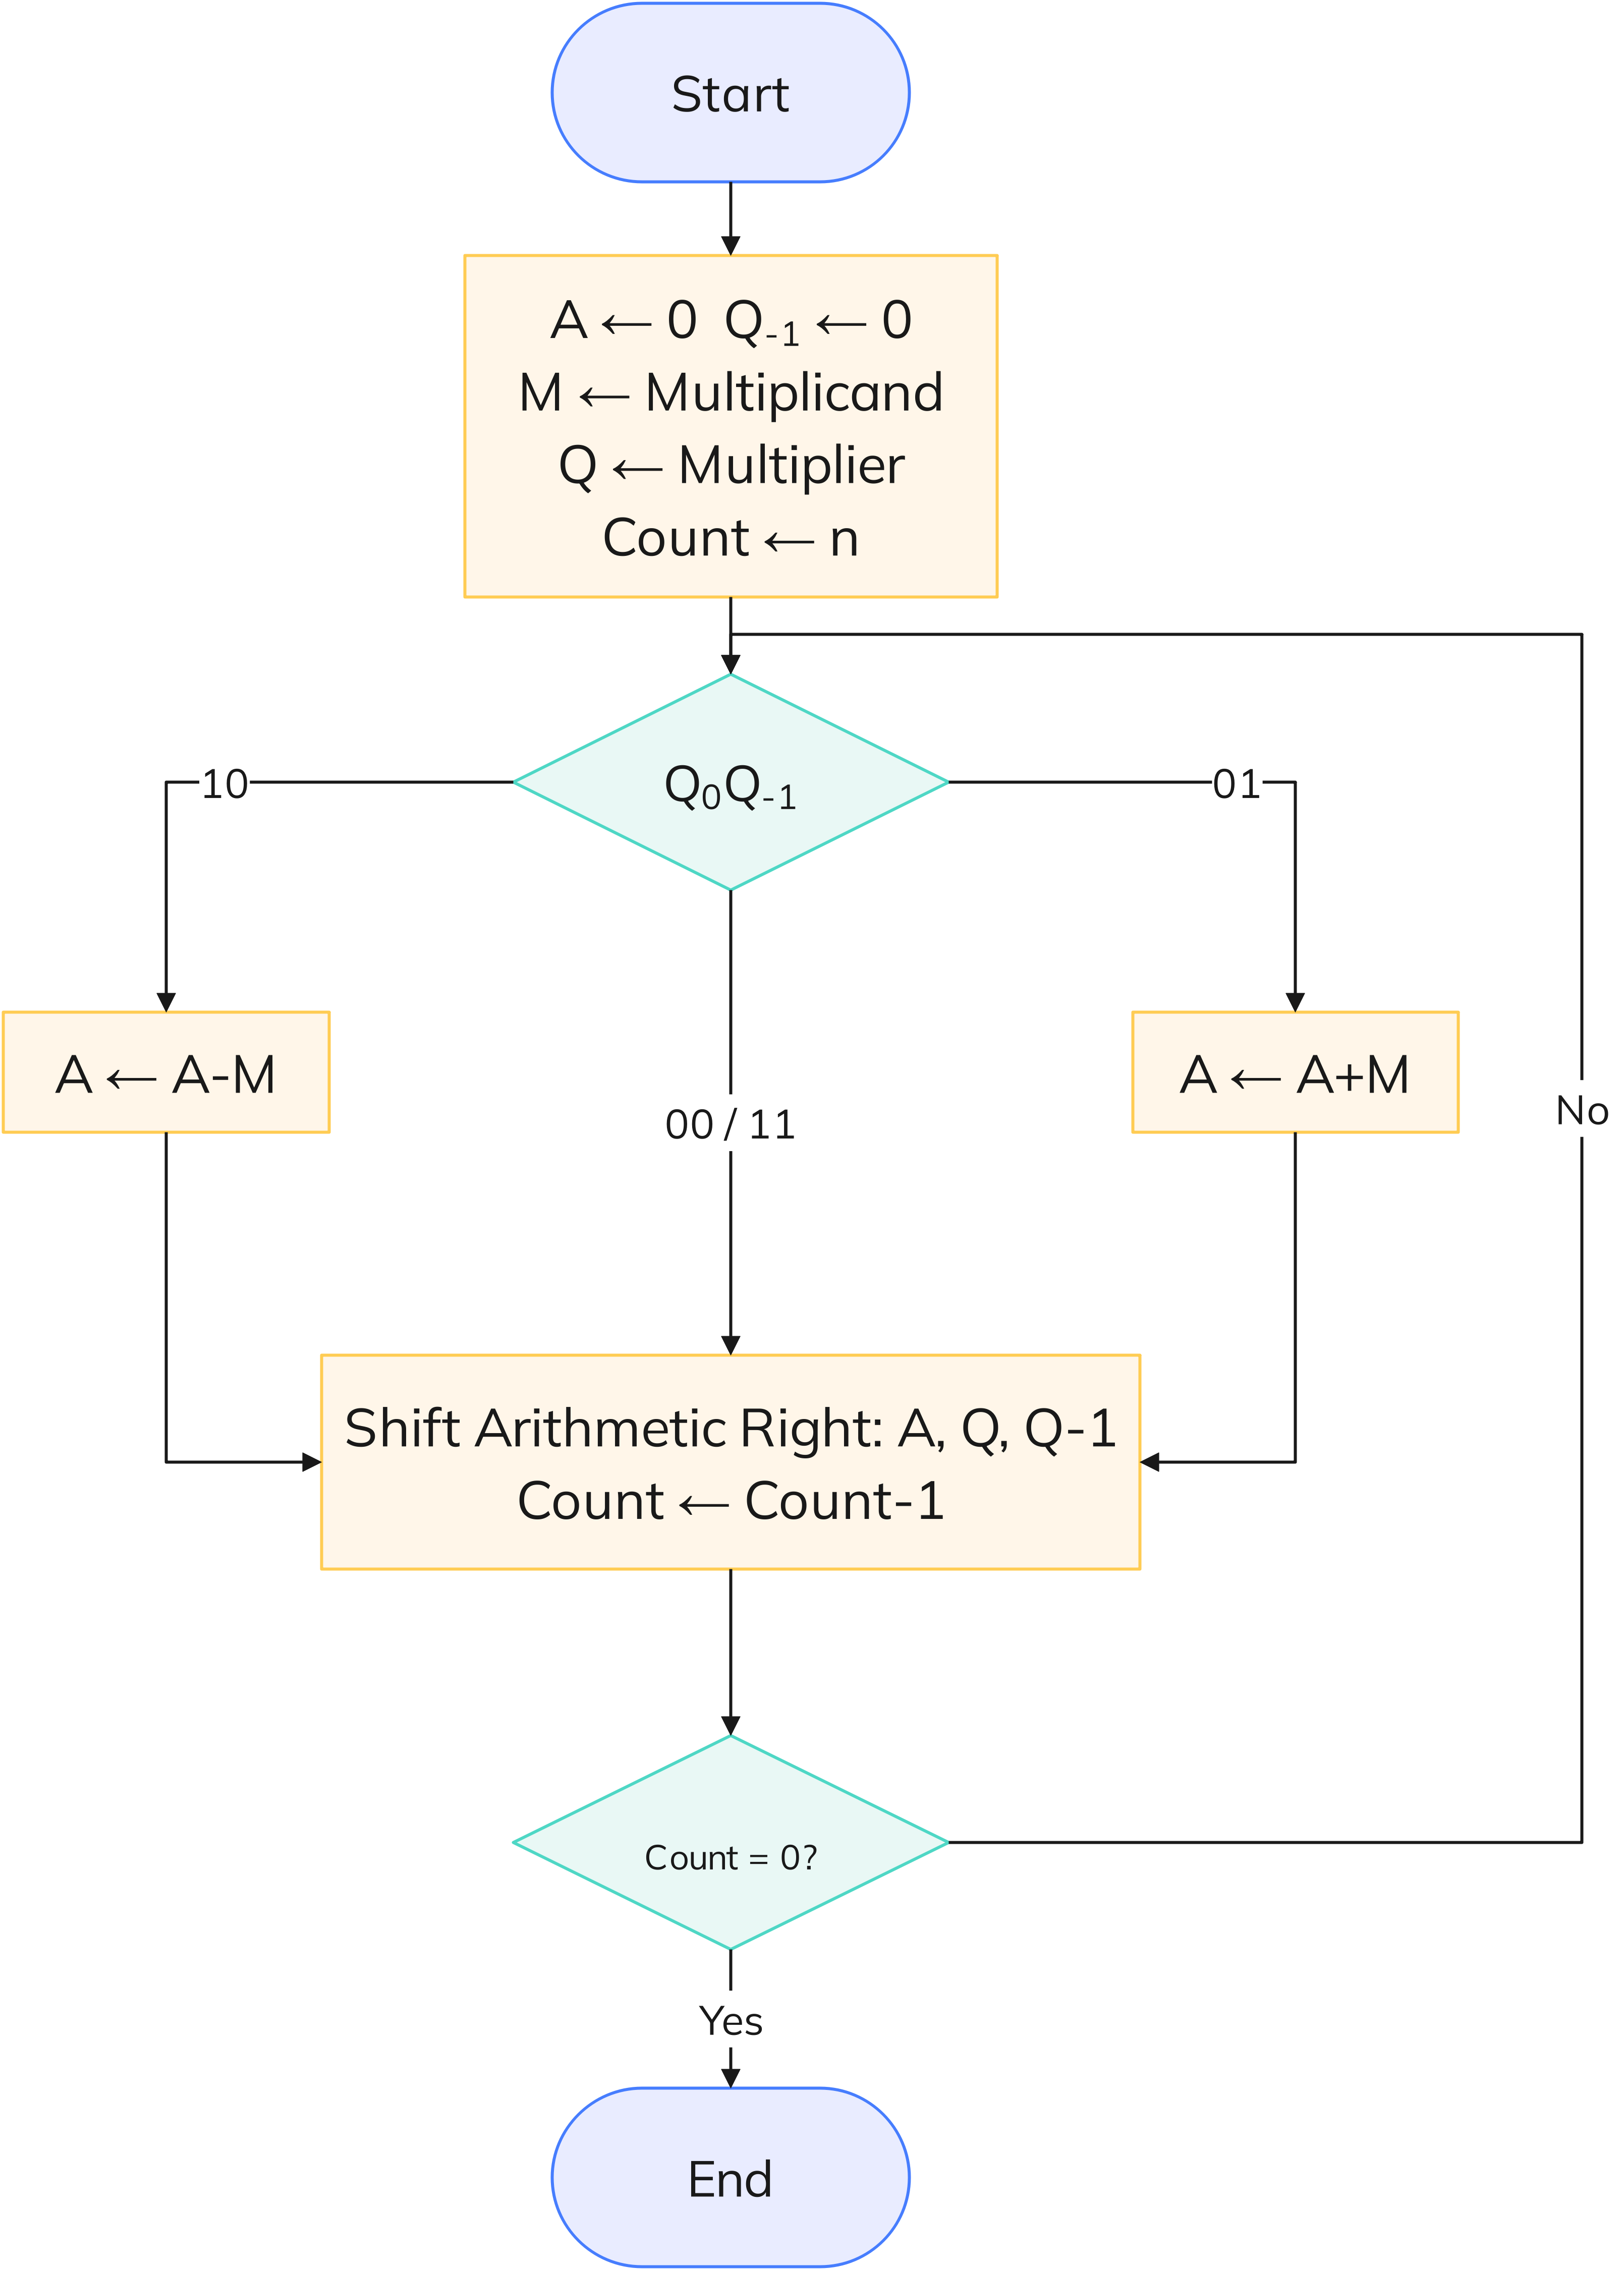
\includegraphics[width=0.45\textwidth]{figures/Booth's Algorithm.png}
\end{figure}
   